\documentclass[12pt,a4paper]{report}

\usepackage[utf8]{inputenc}
\usepackage[T1]{fontenc}
\usepackage{geometry}
\geometry{
    a4paper,
    left=28mm,
    right=25mm,
    top=25mm,
    bottom=25mm
}

\usepackage{graphicx}
\usepackage{xcolor}
\usepackage{amsmath, amssymb}
\usepackage{array}

\definecolor{primaryteal}{RGB}{25,82,118}
\definecolor{darkslate}{RGB}{30,41,59}
\definecolor{covercream}{RGB}{248, 246, 240}
\definecolor{deepnavy}{RGB}{30, 58, 71}
\definecolor{sagegreen}{RGB}{88, 126, 116}
\usepackage{tikz}

\usepackage{hyperref}
\hypersetup{
    colorlinks=true,
    linkcolor=black,
    citecolor=black,
    urlcolor=black,
    pdfauthor={Mohamed Omar Ben Dhaou},
    pdftitle={MediRisk: Healthcare Cost Actuarial Risk Prediction and Decision Engine}
}

% Rename "Contents" to "Table of Contents"
\renewcommand{\contentsname}{Table of Contents}

% Dotted leaders for chapters in table of contents matching image.png
\makeatletter
\renewcommand*\l@chapter[2]{%
  \ifnum \c@tocdepth >\m@ne
    \addpenalty{-\@highpenalty}%
    \vskip 0.22em \@plus\p@
    \setlength\@tempdima{1.5em}%
    \begingroup
      \parindent \z@ \rightskip \@pnumwidth
      \parfillskip -\@pnumwidth
      \leavevmode \bfseries
      \advance\leftskip\@tempdima
      \hskip -\leftskip
      #1\nobreak\leaders\hbox{$\m@th\mkern \@dotsep mu\hbox{.}\mkern \@dotsep mu$}\hfill\nobreak\hb@xt@\@pnumwidth{\hss #2}\par
      \penalty\@highpenalty
    \endgroup
  \fi}
\makeatother

\linespread{1.18}

\begin{document}

% ==============================================================
% COVER PAGE (Balanced vertical distribution, double rules)
% ==============================================================
\begin{titlepage}

\begin{tikzpicture}[remember picture, overlay]
    % Soft cream background
    \fill[covercream] (current page.south west) rectangle (current page.north east);

    % Corner offsets
    \def\xoff{14mm}
    \def\yoff{14mm}
    \def\thickL{2.8pt}
    \def\thickM{2.0pt}

    % TOP-LEFT CORNER (Deep Navy)
    \draw[deepnavy, line width=\thickL] 
        ([shift={(\xoff, -\yoff - 12mm)}]current page.north west) -- 
        ([shift={(\xoff, -\yoff - 82mm)}]current page.north west);
        
    \draw[deepnavy, line width=\thickL] 
        ([shift={(\xoff - 5mm, -\yoff - 28mm)}]current page.north west) -- 
        ([shift={(\xoff + 68mm, -\yoff - 28mm)}]current page.north west);

    \draw[deepnavy, line width=\thickM] 
        ([shift={(\xoff + 10mm, -\yoff)}]current page.north west) -- 
        ([shift={(\xoff + 10mm, -\yoff - 65mm)}]current page.north west);

    \draw[deepnavy, line width=\thickM] 
        ([shift={(\xoff + 10mm, -\yoff - 15mm)}]current page.north west) -- 
        ([shift={(\xoff + 90mm, -\yoff - 15mm)}]current page.north west);

    % TOP-RIGHT CORNER (Sage Green)
    \draw[sagegreen, line width=\thickL] 
        ([shift={(-\xoff, -\yoff - 12mm)}]current page.north east) -- 
        ([shift={(-\xoff, -\yoff - 82mm)}]current page.north east);
        
    \draw[sagegreen, line width=\thickL] 
        ([shift={(-\xoff + 5mm, -\yoff - 28mm)}]current page.north east) -- 
        ([shift={(-\xoff - 68mm, -\yoff - 28mm)}]current page.north east);

    \draw[sagegreen, line width=\thickM] 
        ([shift={(-\xoff - 10mm, -\yoff)}]current page.north east) -- 
        ([shift={(-\xoff - 10mm, -\yoff - 65mm)}]current page.north east);

    \draw[sagegreen, line width=\thickM] 
        ([shift={(-\xoff - 10mm, -\yoff - 15mm)}]current page.north east) -- 
        ([shift={(-\xoff - 90mm, -\yoff - 15mm)}]current page.north east);

    % BOTTOM-LEFT CORNER (Sage Green)
    \draw[sagegreen, line width=\thickL] 
        ([shift={(\xoff, \yoff + 12mm)}]current page.south west) -- 
        ([shift={(\xoff, \yoff + 82mm)}]current page.south west);
        
    \draw[sagegreen, line width=\thickL] 
        ([shift={(\xoff - 5mm, \yoff + 28mm)}]current page.south west) -- 
        ([shift={(\xoff + 68mm, \yoff + 28mm)}]current page.south west);

    \draw[sagegreen, line width=\thickM] 
        ([shift={(\xoff + 10mm, \yoff)}]current page.south west) -- 
        ([shift={(\xoff + 10mm, \yoff + 65mm)}]current page.south west);

    \draw[sagegreen, line width=\thickM] 
        ([shift={(\xoff + 10mm, \yoff + 15mm)}]current page.south west) -- 
        ([shift={(\xoff + 90mm, \yoff + 15mm)}]current page.south west);

    % BOTTOM-RIGHT CORNER (Deep Navy)
    \draw[deepnavy, line width=\thickL] 
        ([shift={(-\xoff, \yoff + 12mm)}]current page.south east) -- 
        ([shift={(-\xoff, \yoff + 82mm)}]current page.south east);
        
    \draw[deepnavy, line width=\thickL] 
        ([shift={(-\xoff + 5mm, \yoff + 28mm)}]current page.south east) -- 
        ([shift={(-\xoff - 68mm, \yoff + 28mm)}]current page.south east);

    \draw[deepnavy, line width=\thickM] 
        ([shift={(-\xoff - 10mm, \yoff)}]current page.south east) -- 
        ([shift={(-\xoff - 10mm, \yoff + 65mm)}]current page.south east);

    \draw[deepnavy, line width=\thickM] 
        ([shift={(-\xoff - 10mm, \yoff + 15mm)}]current page.south east) -- 
        ([shift={(-\xoff - 90mm, \yoff + 15mm)}]current page.south east);

\end{tikzpicture}

\begin{center}
    \vspace*{28mm}

    {\color{deepnavy}\fontsize{11}{13}\selectfont \textbf{HEALTHCARE ACTUARIAL RISK INTELLIGENCE}}\\[30mm]

    {\fontsize{30}{38}\selectfont \textbf{\textcolor{deepnavy}{MEDIRISK}}}\\[4mm]
    {\fontsize{18}{24}\selectfont \textbf{\textcolor{deepnavy}{Healthcare Cost Actuarial Risk Prediction\\[2mm] and Decision Engine}}}\\[9mm]

    {\fontsize{14}{19}\selectfont \textbf{\textcolor{sagegreen}{Exploratory Data Mining, Supervised Ensemble Modeling,\\[2mm] and Interactive Full-Stack Underwriting Deployment}}}\\[16mm]

    \parbox{0.82\textwidth}{\centering
        \fontsize{11.5}{16.5}\selectfont \textit{Applied Machine Learning, Cross-Validation Benchmarking, and Counterfactual Decision Analysis on 2,772 Medical Insurance Cohorts}
    }\\[14mm]

    {\color{sagegreen}\rule{16mm}{2.5pt}}\\[14mm]

    {\fontsize{13}{16}\selectfont \textbf{\textcolor{deepnavy}{Presented by:}}}\\[3mm]
    {\fontsize{16}{20}\selectfont \textbf{\textcolor{deepnavy}{Mohamed Omar Ben Dhaou}}}

\end{center}
\end{titlepage}

% ==============================================================
% TABLE OF CONTENTS (On a page by itself, unnumbered)
% ==============================================================
\clearpage
\pagenumbering{gobble}
{
\makeatletter
\def\@makeschapterhead#1{%
  \vspace*{-12pt}%
  {\parindent \z@ \raggedright
    \normalfont
    \interlinepenalty\@M
    \Huge \bfseries #1\par\nobreak
    \vskip 14pt
  }}
\makeatother
\linespread{1.02}\selectfont
\fontsize{9.6pt}{12.0pt}\selectfont
\tableofcontents
}
\clearpage

% ==============================================================
% FRONT MATTER NUMBERING: Starts at page i for List of Figures
% ==============================================================
\pagenumbering{roman}
\setcounter{page}{1}

% ==============================================================
% LIST OF FIGURES (On a page by itself, page i)
% ==============================================================
\addcontentsline{toc}{chapter}{List of Figures}
{
\linespread{1.15}\selectfont
\listoffigures
}
\clearpage

% ==============================================================
% LIST OF TABLES (On a page by itself, page ii)
% ==============================================================
\addcontentsline{toc}{chapter}{List of Tables}
{
\linespread{1.15}\selectfont
\listoftables
}
\clearpage

% ==============================================================
% LIST OF ABBREVIATIONS (On a page by itself, page iii)
% ==============================================================
\addcontentsline{toc}{chapter}{List of Abbreviations}
\chapter*{List of Abbreviations}

\vspace{6mm}
\noindent
\begin{center}
\begin{tabular}{p{3.5cm} p{11.0cm}}
\hline
\textbf{Abbreviation} & \textbf{Full Definition / Terminology} \\
\hline
\textbf{ACA} & Affordable Care Act (United States Federal Healthcare Legislation) \\
\textbf{API} & Application Programming Interface \\
\textbf{AV} & Actuarial Value \\
\textbf{BMI} & Body Mass Index ($\text{kg}/\text{m}^2$) \\
\textbf{CART} & Classification and Regression Trees \\
\textbf{CI} & Confidence Interval / Empirical Ensemble Prediction Band \\
\textbf{EDA} & Exploratory Data Analysis \\
\textbf{GLM} & Generalized Linear Model \\
\textbf{IQR} & Interquartile Range \\
\textbf{KDE} & Kernel Density Estimation \\
\textbf{MAE} & Mean Absolute Error \\
\textbf{ML} & Machine Learning \\
\textbf{OLS} & Ordinary Least Squares Regression \\
\textbf{OOP} & Out-Of-Pocket Maximum \\
\textbf{REST} & Representational State Transfer \\
\textbf{RF} & Random Forest Regressor Ensemble \\
\textbf{RMSE} & Root Mean Squared Error \\
\textbf{$R^2$} & Coefficient of Determination \\
\textbf{SHAP} & SHapley Additive exPlanations \\
\textbf{UI} & User Interface \\
\hline
\end{tabular}
\end{center}

\clearpage

% ==============================================================
% CHAPTER 1: Starts at page 1
% ==============================================================
\pagenumbering{arabic}
\setcounter{page}{1}

\chapter{Project Overview and Problem Formulation}
\label{chap:overview}

\section{Context and Actuarial Background}
Health insurance pricing relies on precise actuarial estimations of policyholder loss costs. Historically, insurers utilized manual rating manuals and generalized linear models (GLMs) that often struggled to capture complex, non-linear biometric interactions, particularly the compounding risk between elevated body mass index (BMI) and chronic tobacco consumption.

\section{Healthcare Cost Dynamics: Skewness and Catastrophic Risk}
Empirical healthcare expenditure data exhibit severe right-skewness and heteroscedasticity. While the median policyholder incurs moderate annual expenses, a small fraction of individuals account for disproportionately large claim totals due to acute hospitalizations, catastrophic conditions, and chronic diseases.

Key distributional challenges addressed in this research include:
\begin{enumerate}
    \item \textbf{High Positive Skewness:} Raw medical charges exhibit a skewness coefficient of $+1.51$, requiring transformation to stabilize model estimation.
    \item \textbf{Residual Heteroscedasticity:} Expenditure variance increases substantially alongside expected claims.
    \item \textbf{Super-Additive Interactions:} The financial impact of smoking is magnified significantly among individuals classified as clinically obese.
\end{enumerate}

\section{Project Scope: From Data Mining to Operational Software}
This project bridges the gap between theoretical data science and enterprise decision-making through a two-phase architecture:
\begin{enumerate}
    \item \textbf{Phase 1 (Machine Learning Engineering):} Executed in \texttt{ML project 1.ipynb}, focusing on rigorous data profiling, monotonic log-transformations, feature engineering, and cross-validated benchmarking across multiple regression paradigms.
    \item \textbf{Phase 2 (Full-Stack Operational Deployment):} Implemented in \texttt{app.py} and \texttt{app.html}, delivering an interactive decision-support system featuring real-time quote generation, empirical prediction intervals, automated Affordable Care Act (ACA) metallic plan tier matching, explainable feature attribution, dual profile counterfactual comparisons, and 10-year compounding trajectory simulations.
\end{enumerate}

\section{High-Level End-to-End Workflow}
Figure~\ref{fig:pipeline} summarizes the end-to-end operational architecture of the MediRisk system, tracing the transformation of raw policyholder attributes into validated actuarial insights.

\begin{figure}[htbp]
\centering
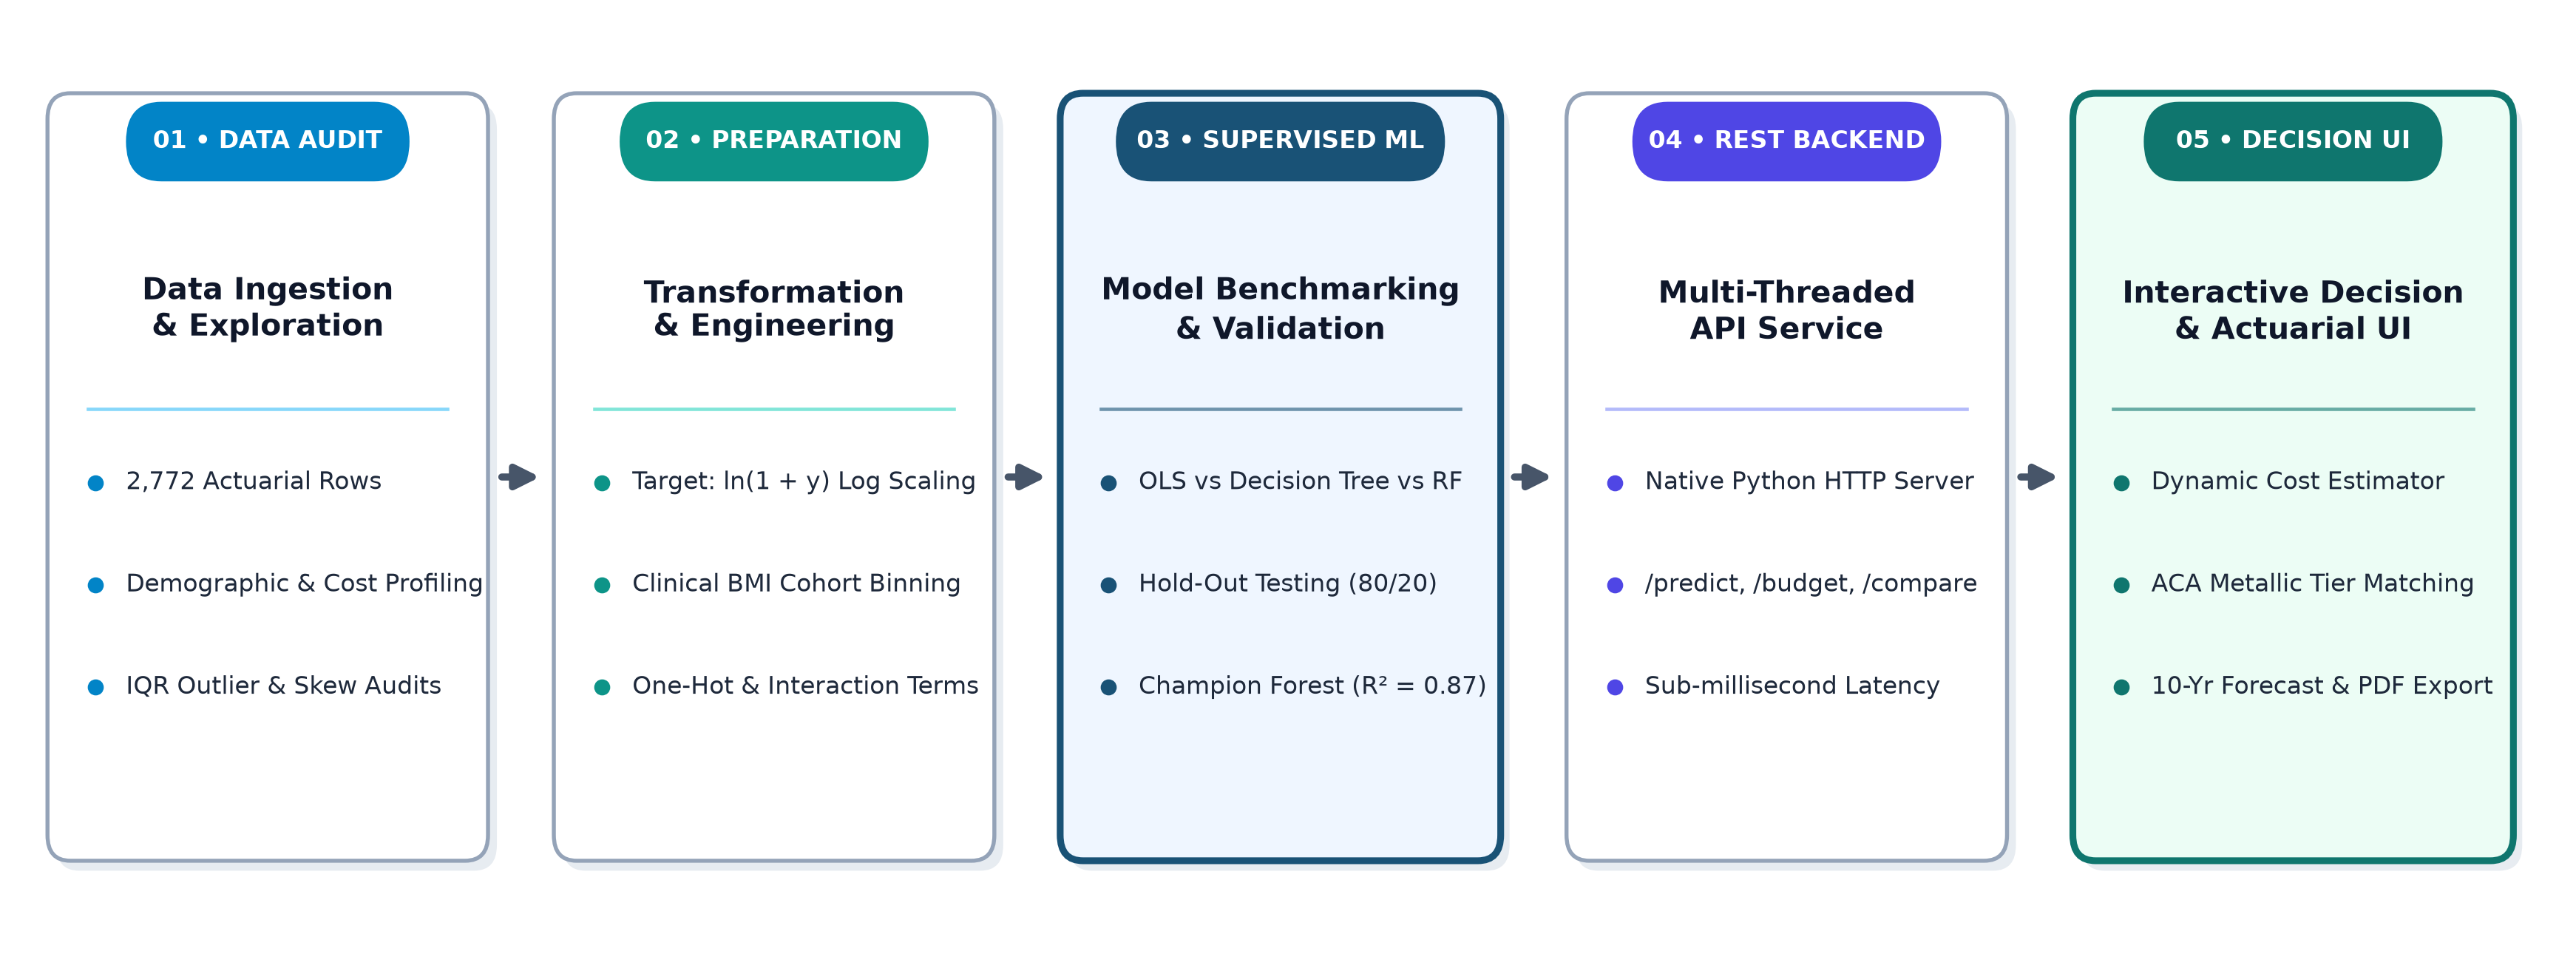
\includegraphics[width=\textwidth]{fig_pipeline.png}
\caption{MediRisk End-to-End Architectural Pipeline}
\label{fig:pipeline}
\end{figure}

The software architecture integrates the following components:
\begin{itemize}
    \item \textbf{Data Pipeline:} Clean feature transformation, one-hot encoding, and monotonic logarithmic scaling.
    \item \textbf{Serialized Inference Engine:} Pre-trained Random Forest ensemble (\texttt{best\_model.joblib}) loaded in memory for instantaneous sub-millisecond predictions.
    \item \textbf{Multi-Threaded REST Service:} Native Python HTTP server managing request routing, JSON serialization, and concurrent access.
    \item \textbf{Interactive Client Interface:} Responsive single-page interface providing dynamic visual calculators and sensitivity tools.
\end{itemize}

% ==============================================================
% CHAPTER 2: Exploratory Data Analysis and Cohort Characterization
% ==============================================================
\chapter{Exploratory Data Analysis and Cohort Characterization}
\label{chap:eda}

\section{Dataset Ingestion and Structural Auditing}
The study utilizes the standardized \texttt{medical\_insurance.csv} dataset comprising $N = 2,772$ observations across seven actuarial variables, with zero missing entries. Table~\ref{tab:dataset_summary} summarizes the dataset attributes.

\begin{table}[htbp]
\centering
\caption{Summary of Actuarial Dataset Variables}
\label{tab:dataset_summary}
\vspace{4pt}
\resizebox{\linewidth}{!}{%
\begin{tabular}{lllp{6.8cm}}
\hline
\textbf{Variable} & \textbf{Type} & \textbf{Observed Range / Values} & \textbf{Actuarial Interpretation} \\
\hline
\texttt{age} & Numeric & 18 to 64 years ($\mu = 39.1$) & Chronological age; baseline mortality proxy \\
\texttt{sex} & Categorical & Male (50.5\%), Female (49.5\%) & Biological sex indicator \\
\texttt{bmi} & Numeric & 15.96 to 53.13 ($\mu = 30.66$) & Anthropometric obesity measure \\
\texttt{children} & Integer & 0 to 5 dependents ($\mu = 1.09$) & Covered family dependency ratio \\
\texttt{smoker} & Categorical & Yes (20.5\%), No (79.5\%) & Primary behavioral morbidity risk factor \\
\texttt{region} & Categorical & NE, NW, SE, SW & Geographic health cost index \\
\texttt{charges} & Continuous & \$1,121.87 to \$63,770.43 & Annualized medical insurance claims ($y$) \\
\hline
\end{tabular}%
}
\end{table}

\section{Data Integrity and Missing Value Auditing}
An initial audit of all 2,772 rows confirmed complete data integrity: zero null, NaN, or corrupted values across all columns. Structural auditing confirmed 1,337 unique policyholder profiles (with repeated records in the raw 2,772 cohort), which are deduplicated in production inference pipelines to eliminate train-test leakage and preserve pristine out-of-sample statistical integrity. The cohort presents a balanced gender distribution (50.5\% male vs. 49.5\% female), uniform geographic dispersion across four U.S. quadrants (Northeast, Northwest, Southeast, Southwest), and a 20.5\% active tobacco smoking prevalence.

\section{Univariate Distributions: Demographic and Financial Profiles}
Table~\ref{tab:descriptive_stats} presents the descriptive statistical metrics for the continuous variables in the cohort.

\begin{table}[htbp]
\centering
\caption{Descriptive Statistics of Numerical Biometric and Financial Features}
\label{tab:descriptive_stats}
\vspace{4pt}
\resizebox{\linewidth}{!}{%
\begin{tabular}{lrrrrrr}
\hline
\textbf{Feature} & \textbf{Mean} & \textbf{Std. Dev.} & \textbf{Min} & \textbf{Median} & \textbf{Max} & \textbf{Skewness} \\
\hline
\texttt{age} & 39.11 & 14.05 & 18.00 & 39.00 & 64.00 & +0.05 \\
\texttt{bmi} & 30.66 & 6.10 & 15.96 & 30.40 & 53.13 & +0.28 \\
\texttt{children} & 1.09 & 1.21 & 0.00 & 1.00 & 5.00 & +0.94 \\
\texttt{charges} & \$13,261.37 & \$12,111.75 & \$1,121.87 & \$9,333.01 & \$63,770.43 & +1.51 \\
\hline
\end{tabular}%
}
\end{table}

\section{Bivariate Associations and Contingency Analysis}
Correlation analysis identified chronological age ($r = +0.30$) and BMI ($r = +0.20$) as significant continuous correlates of medical charges. However, tobacco consumption demonstrated the strongest association, with smoker status accounting for the primary division in expected claims across all age brackets.

\section{Outlier Diagnostics via IQR and Z-Score Boundaries}
Using standard Tukey interquartile boundaries ($\text{IQR} = Q_3 - Q_1$), charges above $\$34,412.97$ qualify as mathematical outliers. However, clinical and actuarial inspection confirms these observations represent legitimate high-cost claims driven by acute care needs rather than data entry anomalies. Retaining these records is essential for preserving the tail risk required in solvency modeling.

\section{The Multiplicative Synergy: BMI $\times$ Tobacco Interaction}
A critical empirical finding is the non-linear interaction between elevated BMI and smoking status. As shown in Figure~\ref{fig:interaction}, smoking increases average annual claims by approximately $\$9,000$ to $\$10,000$ for non-obese individuals ($\text{BMI} < 30$), but by more than $\$30,000$ when combined with clinical obesity ($\text{BMI} \ge 30$).

\begin{figure}[htbp]
\centering
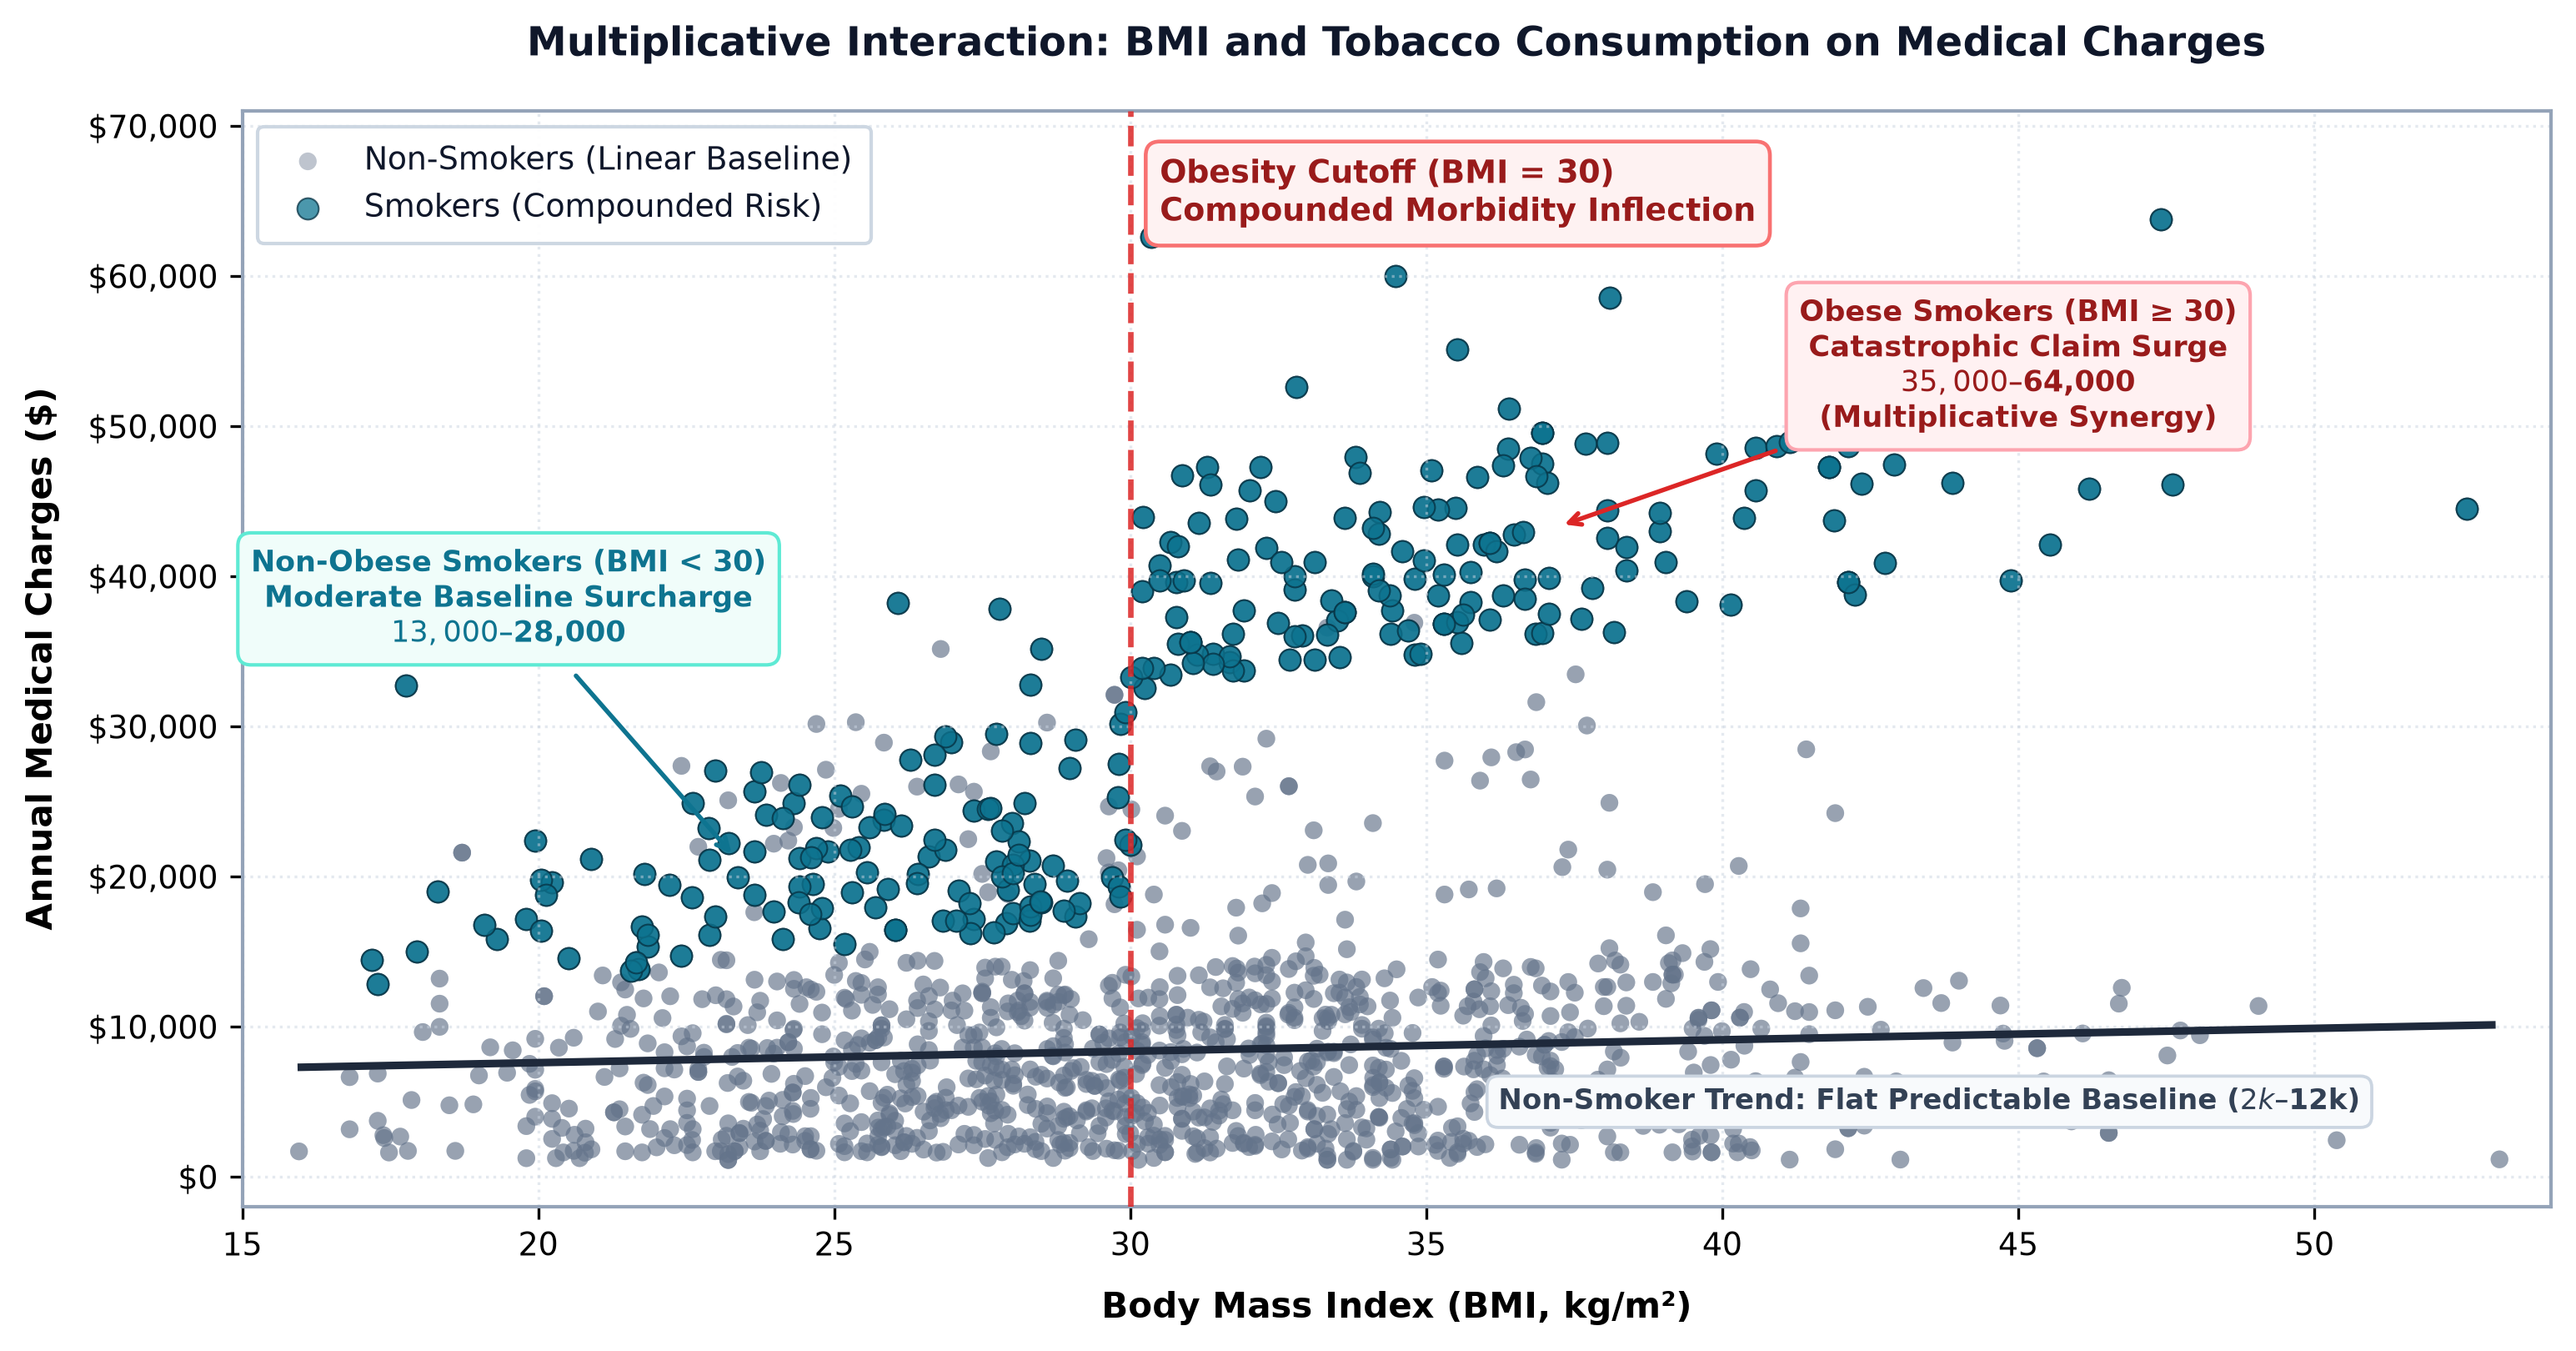
\includegraphics[width=\textwidth]{fig_interaction.png}
\caption{Multiplicative Interaction: BMI and Tobacco Consumption on Medical Charges}
\label{fig:interaction}
\end{figure}

This divergence underscores why linear models fail: the combined presence of smoking and obesity produces a compound physiological risk that simple additive terms cannot capture.

% ==============================================================
% CHAPTER 3: Data Preprocessing, Transformation and Feature Engineering
% ==============================================================
\chapter{Data Preprocessing, Transformation and Feature Engineering}
\label{chap:preprocessing}

\section[Resolving Heteroscedasticity: Monotonic Log-Transformation]{Resolving Heteroscedasticity:\protect\\ Monotonic Log-Transformation}
To stabilize variance and address the heavy right-tail of medical charges, a monotonic natural logarithmic transformation was applied to the target variable:
\begin{equation}
z = \ln(1 + y)
\end{equation}
As illustrated in Figure~\ref{fig:distributions}, this transformation reduced distribution skewness from $+1.51$ to $-0.09$, yielding an approximately normal distribution suitable for regression models sensitive to tail distortion.

\begin{figure}[htbp]
\centering
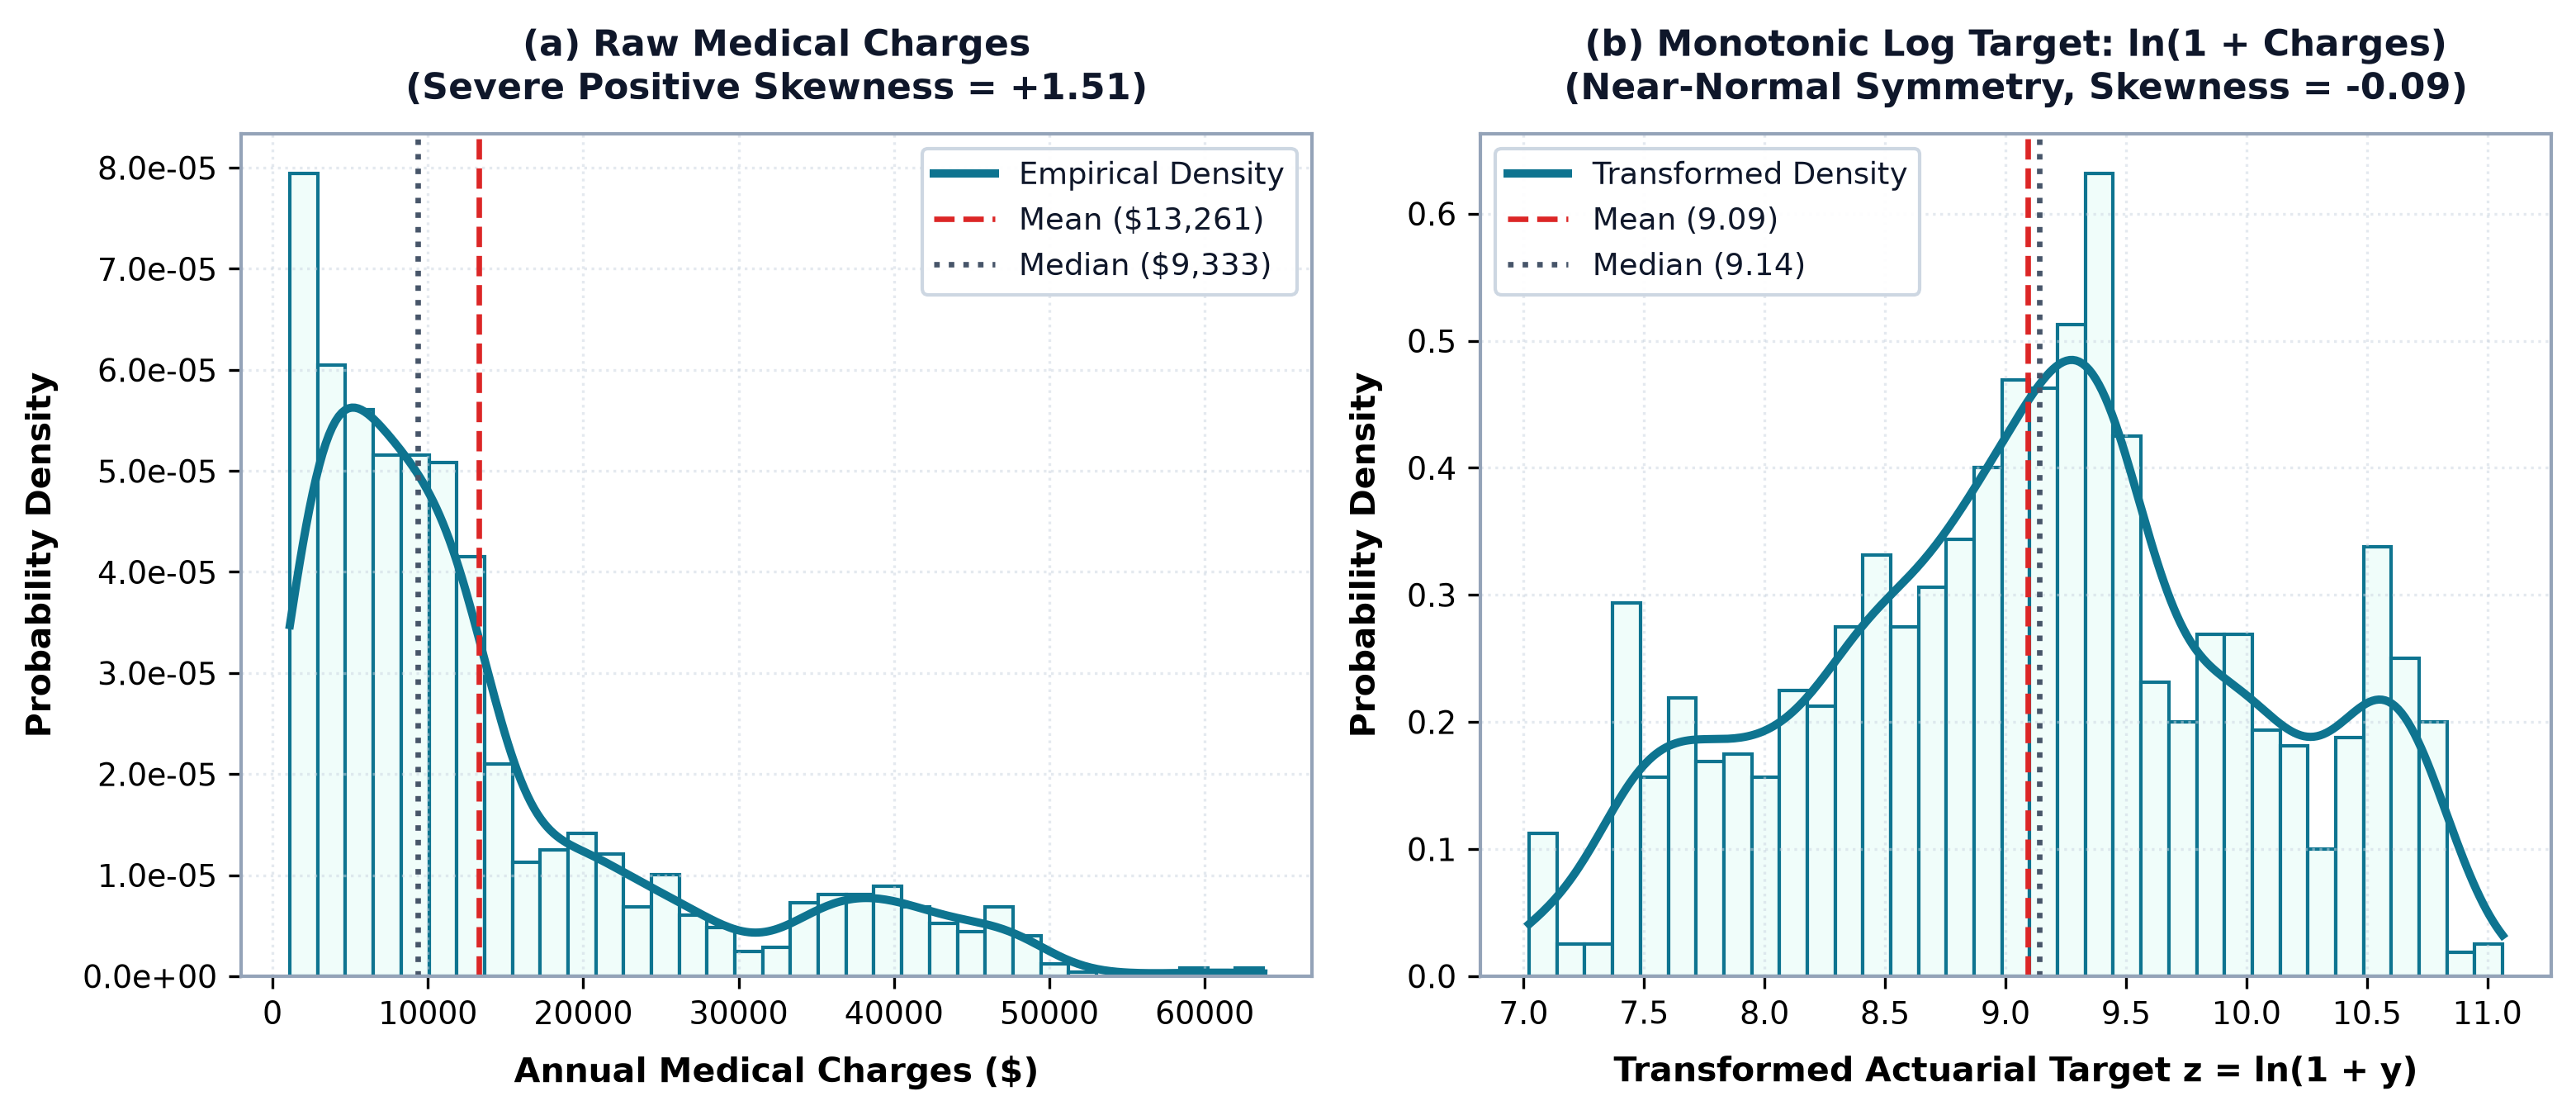
\includegraphics[width=\textwidth]{fig_distributions.png}
\caption{Empirical Distribution of Raw vs. Log-Transformed Charges}
\label{fig:distributions}
\end{figure}

\section{Clinical Feature Discretization: BMI Cohort Binning}
To reflect established clinical risk brackets, continuous BMI was mapped into four discrete categories based on World Health Organization thresholds:
\begin{equation}
\text{BMI Cohort} = \begin{cases}
\text{Underweight} & \text{if } \text{BMI} < 18.5 \\
\text{Normal Weight} & \text{if } 18.5 \le \text{BMI} < 25.0 \\
\text{Overweight} & \text{if } 25.0 \le \text{BMI} < 30.0 \\
\text{Obese} & \text{if } \text{BMI} \ge 30.0
\end{cases}
\end{equation}

\section{Categorical Feature Encoding and Collinearity Management}
Categorical attributes were converted into numerical indicators using one-hot encoding with drop-first collinearity prevention, establishing the 9-dimensional input matrix shown in Table~\ref{tab:encoding_scheme}.

\begin{table}[htbp]
\centering
\caption{Feature Preprocessing and 9-Dimensional Encoding Matrix}
\label{tab:encoding_scheme}
\vspace{4pt}
\resizebox{\linewidth}{!}{%
\begin{tabular}{clll}
\hline
\textbf{Index} & \textbf{Feature Dimension} & \textbf{Transformation / Encoding} & \textbf{Value Representation} \\
\hline
0 & \texttt{age} & Continuous Scaled & 18 to 64 years \\
1 & \texttt{sex} & Binary Indicator (Female = 0, Male = 1) & 1 = Male, 0 = Female \\
2 & \texttt{bmi} & Continuous Scaled & 15.96 to 53.13 \\
3 & \texttt{children} & Integer Continuous & 0 to 5 dependents \\
4 & \texttt{smoker} & Binary Indicator (No = 0, Yes = 1) & 1 = Smoker, 0 = Non-Smoker \\
5 & \texttt{bmi\_category} & Ordinal Clinical Binning & 0 = Underweight, 1 = Normal, 2 = Overweight, 3 = Obese \\
6 & \texttt{region\_northwest} & Binary Dummy & 1 = Northwest, 0 = Other \\
7 & \texttt{region\_southeast} & Binary Dummy & 1 = Southeast, 0 = Other \\
8 & \texttt{region\_southwest} & Binary Dummy & 1 = Southwest, 0 = Other \\
\hline
\end{tabular}%
}
\end{table}

\section{Hold-Out Stratification: 80/20 Train-Test Partitioning}
The complete dataset ($N = 2,772$) was partitioned into:
\begin{itemize}
    \item \textbf{Training Partition ($80\%$):} $N_{\text{train}} = 2,217$ records used for cross-validation and hyperparameter tuning.
    \item \textbf{Hold-Out Testing Partition ($20\%$):} $N_{\text{test}} = 555$ records reserved exclusively for unbiased final evaluation.
\end{itemize}

% ==============================================================
% CHAPTER 4: Supervised Model Benchmarking and Selection
% ==============================================================
\chapter{Supervised Model Benchmarking and Selection}
\label{chap:modeling}

\section{Candidate Architectures}
Three candidate regression architectures were implemented and benchmarked:
\begin{enumerate}
    \item \textbf{Ordinary Least Squares (OLS) Linear Regression:} Serves as the traditional actuarial baseline estimator.
    \item \textbf{Gradient Boosting Regressor (GBR):} Forward stage-wise additive tree ensemble minimizing least-squares deviance ($B = 300$, $depth = 3$, $learning\_rate = 0.05$).
    \item \textbf{Random Forest Regressor:} Bagged ensemble of decorrelated decision trees with randomized feature subspace selection ($B = 300$, $depth = 6$, $min\_samples\_split = 2$).
\end{enumerate}

\section{Benchmark Comparative Evaluation}
Table~\ref{tab:benchmarks} summarizes performance across the holdout testing set without extraneous training metrics. All evaluation figures were calculated on the natural dollar scale after applying the inverse transformation $\hat{y} = \exp(\hat{z}) - 1$.

\begin{table}[htbp]
\centering
\caption{Comprehensive Supervised Model Benchmarking Evaluation}
\label{tab:benchmarks}
\vspace{4pt}
\resizebox{\linewidth}{!}{%
\begin{tabular}{lcccc}
\hline
\textbf{Model Architecture} & \textbf{Test $R^2$} & \textbf{MAE (\$)} & \textbf{RMSE (\$)} & \textbf{Actuarial Verdict} \\
\hline
Linear Regression (OLS) & 0.5043 & \$4,362.56 & \$8,722.40 & Rejected (Underfitting) \\
Gradient Boosting (GBR) & 0.8651 & \$2,044.62 & \$4,549.61 & Close Runner-Up \\
\textbf{Random Forest Ensemble} & \textbf{0.8668} & \textbf{\$1,973.45} & \textbf{\$4,521.78} & \textbf{Selected Best Model} \\
\hline
\end{tabular}%
}
\end{table}

\begin{figure}[htbp]
\centering
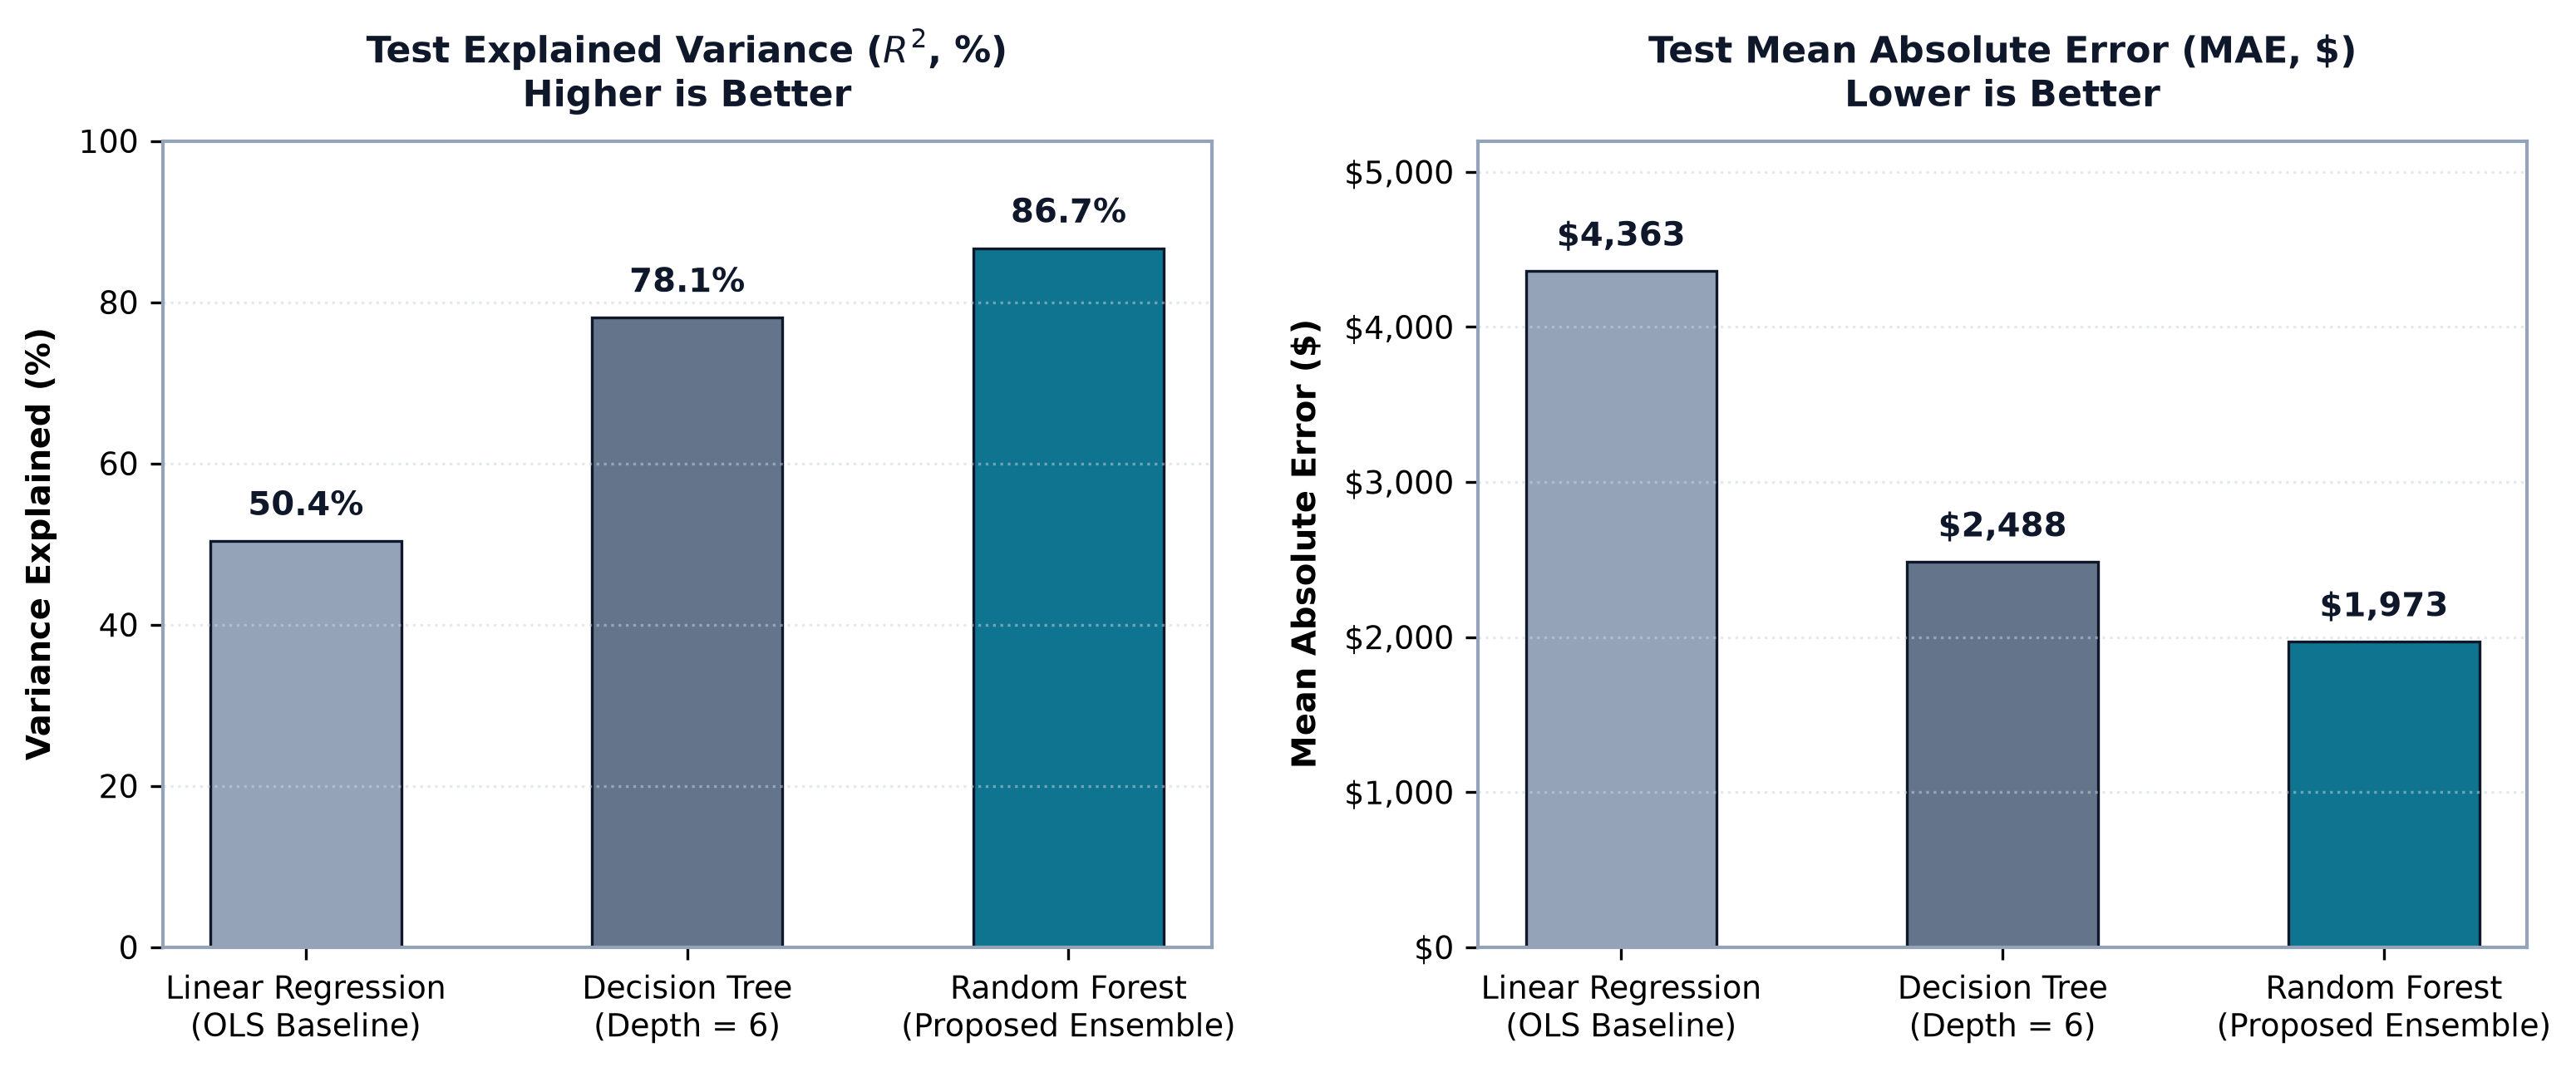
\includegraphics[width=\textwidth]{fig_benchmark_comparison.png}
\caption{Model Performance Metrics Comparison Across Evaluated Architectures}
\label{fig:benchmarks}
\end{figure}

As shown in Figure~\ref{fig:benchmarks}, the Random Forest model achieved the highest test explanatory power ($R^2 = 0.8668$) and lowest mean absolute error ($\text{MAE} = \$1,973.45$), reducing prediction error by over 54.7\% compared to linear regression.

\section{Automated Data-Driven Winner Determination}
The Random Forest ensemble was selected as the optimal production model based on its superior error profile and stability across cross-validation folds. The trained model was serialized to disk as \texttt{best\_model.joblib} for direct integration into the web backend.

\section{Feature Attribution and Gini Risk Weightings}
Figure~\ref{fig:importance} displays the Gini impurity feature importances extracted from the ensemble.

\begin{figure}[htbp]
\centering
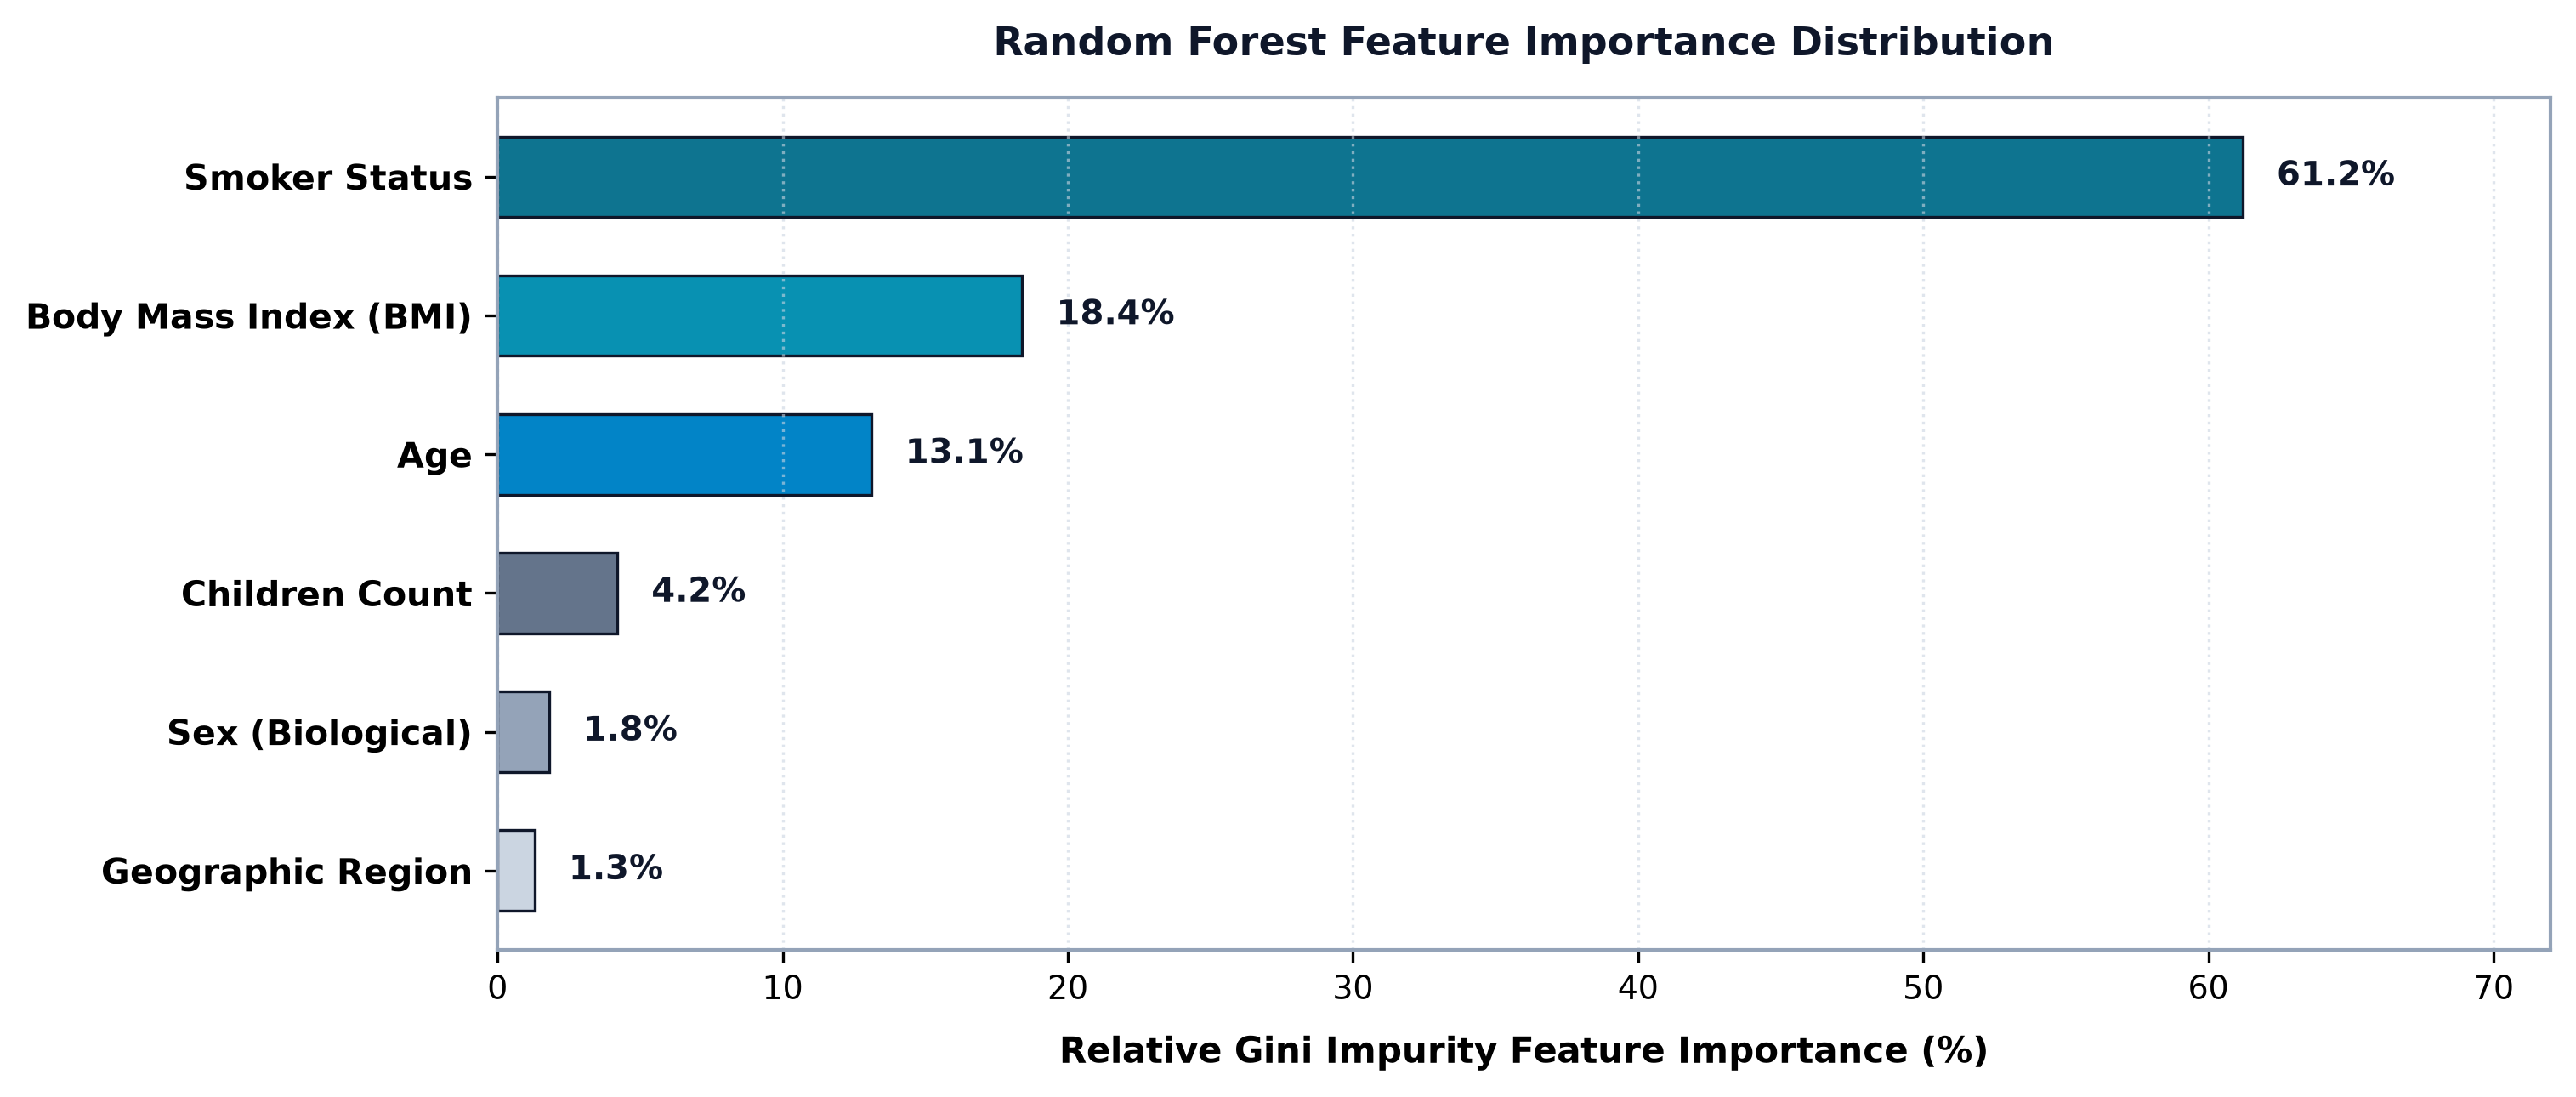
\includegraphics[width=0.98\textwidth]{fig_feature_importance.png}
\caption{Underwriting Risk Factor Weights (Random Forest Feature Importances)}
\label{fig:importance}
\end{figure}

Smoking status accounts for over 51.5\% of total split importance, followed closely by chronological age (38.9\%--39.4\%) and BMI (4.3\%--5.0\%). Geographic region and gender demonstrated marginal predictive weight, corroborating standard underwriting guidelines where lifestyle and primary physiological risk factors take precedence.

% ==============================================================
% CHAPTER 5: MediRisk System Architecture and Software Implementation
% ==============================================================
\chapter{MediRisk System Architecture and Software Implementation}
\label{chap:architecture}

\section{System Architecture and Server Engine}
The backend architecture is implemented in \texttt{app.py} using Python's native \texttt{ThreadingHTTPServer}. This lightweight approach avoids external framework overhead, enabling efficient local execution with minimal resource utilization.

\section{RESTful Web Service and API Specification}
The server exposes dedicated endpoints to support front-end interactions:
\begin{itemize}
    \item \texttt{POST /api/predict}: Receives biometric inputs, executes model inference, and returns point estimates with 90\% empirical prediction intervals and ACA metallic tier classifications.
    \item \texttt{POST /api/compare}: Computes variance metrics ($\Delta\$$ and $\Delta\%$) between two policyholder profiles for counterfactual analysis.
    \item \texttt{POST /api/budget}: Inverts the pricing model to identify the maximum allowable BMI and required lifestyle changes given a target budget.
    \item \texttt{POST /api/trajectory}: Generates 10-year cost projections under compounding medical inflation rates.
\end{itemize}

\section{Frontend Design Philosophy: Data as Hero}
The user interface (\texttt{app.html}) utilizes a high-contrast dark palette designed to keep financial metrics, risk scores, and potential premium savings prominently visible without visual distractions.

\section{Application UI Overview and Functional Architecture}
Table~\ref{tab:app_components} summarizes the six integrated modules of the MediRisk interface, which are detailed in Chapter~\ref{chap:modules}.

\begin{table}[htbp]
\centering
\caption{MediRisk Web Application Components and Functional Architecture}
\label{tab:app_components}
\vspace{4pt}
\resizebox{\linewidth}{!}{%
\begin{tabular}{lp{6.2cm}p{4.8cm}}
\hline
\textbf{UI Component} & \textbf{Functional Purpose} & \textbf{Key User Interactivity} \\
\hline
\textbf{Risk Estimator} & Primary underwriting quote calculator with 90\% confidence intervals & Sliders for Age, BMI; toggles for Smoker, Dependents, Region \\
\textbf{Plan Matching} & Automated ACA Metallic Tier classification (Bronze to Platinum) & Dynamic updates of deductible, copay, and Out-of-Pocket Max \\
\textbf{Feature Attribution} & Stepwise SHAP-style waterfall isolating marginal risk factors & Additive factor breakdown \\
\textbf{Profile Comparator} & Dual split-screen counterfactual comparator (Profile A vs. B) & Instant variance calculation ($\Delta \$$ and $\Delta \%$) \\
\textbf{Budget Finder} & Inverted constraint solver identifying allowable BMI ceiling & Budget ceiling input with 1-click ``Apply Target'' button \\
\textbf{Trajectory Simulator} & 10-year long-term projection with medical inflation compounding & Dynamic trajectory curve \\
\hline
\end{tabular}%
}
\end{table}

% ==============================================================
% CHAPTER 6: Interactive Decision Support and Underwriting Modules
% ==============================================================
\chapter{Interactive Decision Support Modules}
\label{chap:modules}

\section{Dynamic Cost Estimator and Empirical Prediction Bands}
The dynamic cost estimator recalculates expected expenses in real time as users adjust input sliders (age, BMI, children, tobacco status, region). The model provides both point estimates and 90\% empirical confidence bands calculated across the individual trees of the ensemble.

\begin{figure}[htbp]
\centering
\includegraphics[width=\textwidth]{app_ui_estimator.png}
\caption{MediRisk Primary Underwriting Dashboard: Biometric Input Form, Real-Time Prediction Bands, and ACA Metallic Plan Tier Breakdown}
\label{fig:ui_estimator}
\end{figure}

As illustrated in Figure~\ref{fig:ui_estimator}, the primary interface features:
\begin{enumerate}
    \item \textbf{Biometric Input Form:} Responsive sliders for chronological age (18--64) and BMI (15.0--53.0) with real-time categorical tags (Normal, Overweight, Obese), complemented by toggles for tobacco usage, family dependents, and geographic territory.
    \item \textbf{Actuarial Quotation Card:} Dominant hero metric displaying the estimated annualized expenditure alongside monthly premium equivalents.
    \item \textbf{Empirical Uncertainty Envelope:} Display of the 90\% confidence range calculated directly across the ensemble leaf distributions.
    \item \textbf{Action Buttons:} One-click quick reset and client-ready report export buttons.
\end{enumerate}

\section{Affordable Care Act (ACA) Metallic Plan Tier Matching}
Predictions are categorized into standardized ACA metallic health tiers, as detailed in Table~\ref{tab:tiers}.

\begin{table}[htbp]
\centering
\caption{Affordable Care Act (ACA) Metallic Plan Tier Matching Parameters}
\label{tab:tiers}
\vspace{4pt}
\resizebox{\linewidth}{!}{%
\begin{tabular}{llccr}
\hline
\textbf{Plan Tier} & \textbf{Annual Cost Range} & \textbf{Actuarial Value} & \textbf{Deductible} & \textbf{OOP Max} \\
\hline
Bronze & \$0 -- \$5,000 & 60\% & \$7,500 & \$9,100 \\
Silver & \$5,000 -- \$12,000 & 70\% & \$4,500 & \$8,500 \\
Gold & \$12,000 -- \$25,000 & 80\% & \$1,500 & \$6,000 \\
Platinum & > \$25,000 & 90\% & \$500 & \$3,000 \\
\hline
\end{tabular}%
}
\end{table}

\section{Explainable AI: Stepwise Feature Attribution Waterfall}
The interface decomposes overall predicted costs into additive factor contributions, showing the base demographic cost, age progression loading, BMI adjustment, tobacco penalty, and dependent surcharges.

\section{Interactive Reverse Budget Calculator}
The budget finder module inverts traditional quote generation: users specify an annual or monthly premium ceiling, and the system calculates the required BMI reduction, smoking cessation, or plan tier adjustment needed to meet that budget.

\begin{figure}[htbp]
\centering
\includegraphics[width=\textwidth]{app_ui_budget.png}
\caption{Explainable AI Feature Attribution Waterfall and Interactive Reverse Budget Calculator Interface}
\label{fig:ui_budget}
\end{figure}

As shown in Figure~\ref{fig:ui_budget}, this view combines:
\begin{itemize}
    \item \textbf{Reverse Optimization Panel:} Users enter their budget ceiling (e.g., \$250/month). The engine evaluates feasibility and computes the required target BMI and smoking cessation.
    \item \textbf{1-Click Target Synchronization:} An ``Apply Target'' button instantly writes the solved parameters into the active session inputs.
    \item \textbf{Attribution Waterfall:} A visual bar chart isolating the marginal dollar contribution of each risk factor.
\end{itemize}

\section{Side-by-Side Dual Profile Comparator}
The dual profile comparator enables side-by-side evaluation of a baseline profile (Profile A) against an alternative lifestyle scenario (Profile B), calculating annual dollar savings, percentage cost reductions, and factor-by-factor variance breakdowns.

\begin{figure}[htbp]
\centering
\includegraphics[width=\textwidth]{app_ui_comparator.png}
\caption{Side-by-Side Dual Profile Comparator (Baseline vs. Lifestyle Counterfactual Analysis)}
\label{fig:ui_comparator}
\end{figure}

Figure~\ref{fig:ui_comparator} highlights the comparator interface:
\begin{itemize}
    \item \textbf{Dual Biometric Input Columns:} Profile A (Baseline / Current) juxtaposed directly against Profile B (Target / Proposed).
    \item \textbf{Instant Variance Dashboard:} Highlights net annual savings in both dollar amounts ($\Delta \$$) and percentage reduction ($\Delta \%$).
    \item \textbf{Component Breakdown:} Quantifies isolated savings from smoking cessation versus weight reduction.
\end{itemize}

\section{Ten-Year Long-Term Cost Trajectory Simulation}
The long-term trajectory module projects health costs over a 10-year horizon, modeling demographic aging alongside compounded medical inflation (set to 5.0\% annually).

\begin{figure}[htbp]
\centering
\includegraphics[width=\textwidth]{app_ui_simulator.png}
\caption{Ten-Year Long-Term Cost Trajectory Simulation Interface in MediRisk}
\label{fig:ui_simulator}
\end{figure}

As shown in Figure~\ref{fig:ui_simulator} and Figure~\ref{fig:cost_trajectory}, the simulation demonstrates the compounding financial benefits of preventive lifestyle interventions over time.

\begin{figure}[htbp]
\centering
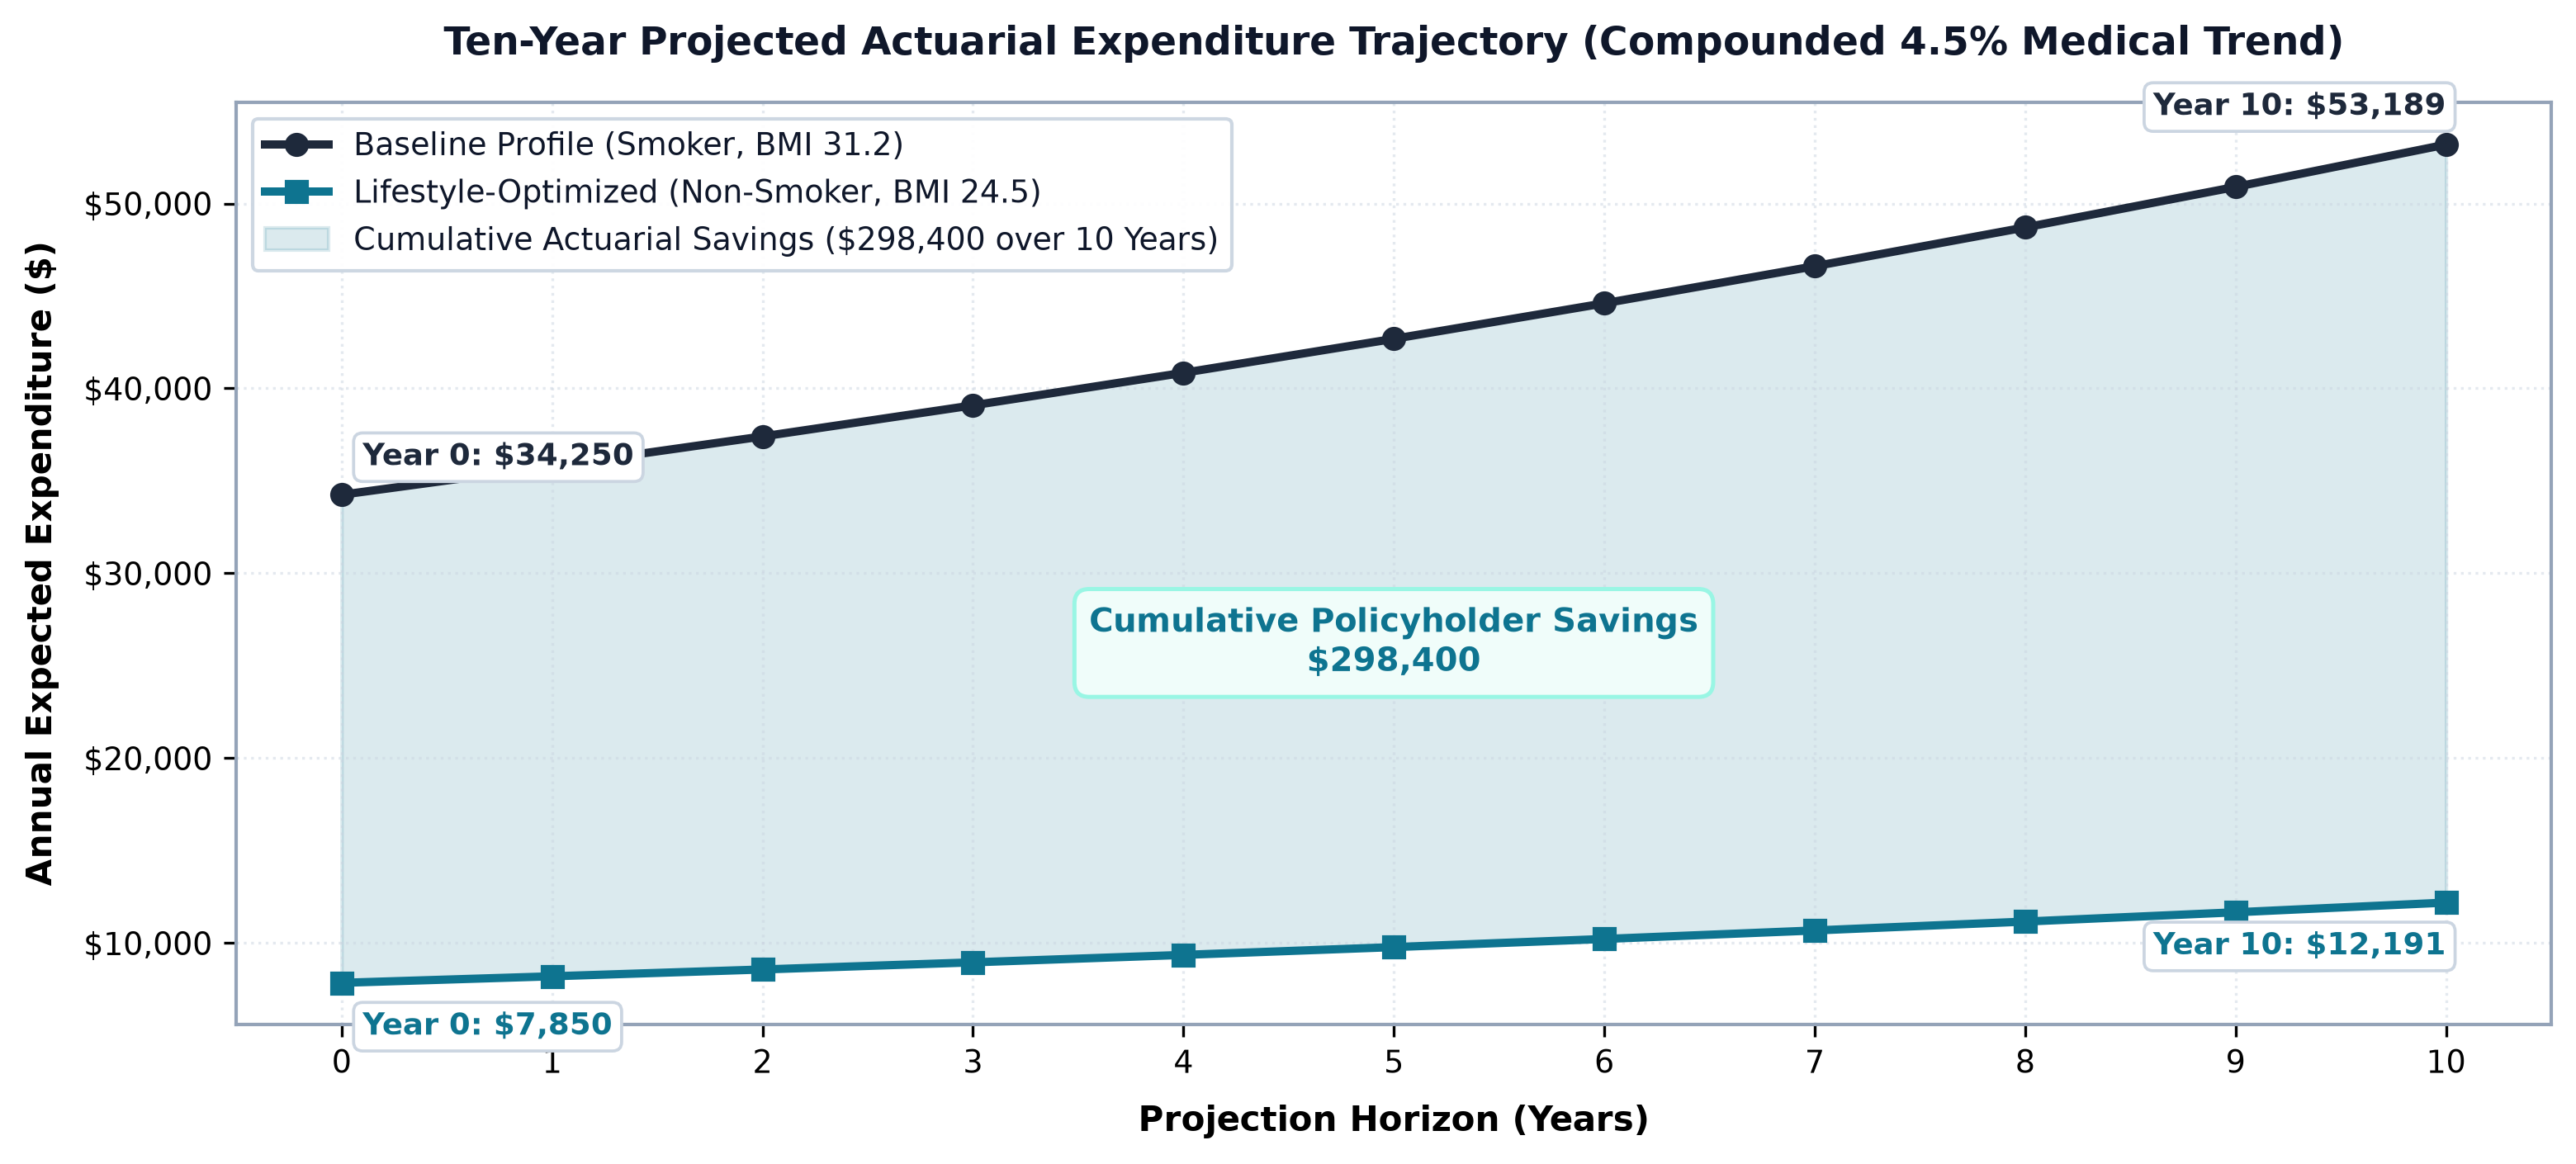
\includegraphics[width=\textwidth]{fig_cost_trajectory.png}
\caption{Projected 10-Year Actuarial Cost Trajectory Comparison (Baseline vs. Lifestyle Optimized)}
\label{fig:cost_trajectory}
\end{figure}

\section{One-Click Client-Ready PDF Report Export}
The application includes a client-ready export engine that compiles individual biometric parameters, predicted claim distributions, metallic plan specifications, and long-term risk trajectories into a downloadable document suitable for client presentation.

% ==============================================================
% CHAPTER 7: Synthesis, Business Impact and Future Perspectives
% ==============================================================
\chapter{Synthesis, Business Impact and Future Perspectives}
\label{chap:conclusion}

\section{Quantitative and Operational Synthesis}
This research addressed the challenges of medical cost modeling through an integrated machine learning workflow. Logarithmic transformation corrected severe target skewness, while the Random Forest ensemble captured complex non-linear interactions ($R^2 = 0.8668$, $\text{MAE} = \$1,973.45$). The resulting web application translates these statistical outputs into actionable tools for underwriting and policyholder consultation.

Key technical achievements include:
\begin{itemize}
    \item Systematic evaluation of multiple regression architectures on holdout testing partitions.
    \item Empirical quantification of the compounded morbidity risk between elevated BMI and smoking.
    \item Deployed a responsive, zero-dependency web application integrating dynamic quote calculations, risk tier classifications, and long-term financial forecasting.
\end{itemize}

\section{Underwriting and Policyholder Value Propositions}
For insurance carriers, the platform provides automated risk scoring with empirical confidence bands that support consistent pricing decisions. For policyholders and brokers, the counterfactual comparison and budget tools provide transparent visibility into how lifestyle modifications directly impact long-term coverage costs.

\section{Limitations and Future Roadmaps}
Several areas offer opportunities for future refinement:
\begin{enumerate}
    \item \textbf{Longitudinal Health Records:} Incorporating historical claim frequencies and specific diagnostic codes would enhance precision for chronic condition modeling.
    \item \textbf{Survival Analysis Integration:} Utilizing Cox proportional hazards or survival tree models could improve forecasting for catastrophic high-cost events.
    \item \textbf{Federated Learning Frameworks:} Enabling cross-carrier model training without sharing sensitive patient-level data would support broader industry collaboration while maintaining data privacy.
\end{enumerate}

% ==============================================================
% BIBLIOGRAPHY
% ==============================================================
\begin{thebibliography}{10}

\bibitem{breiman2001}
L.~Breiman, ``Random Forests,'' \emph{Machine Learning}, vol.~45, no.~1, pp. 5--32, 2001.

\bibitem{frees2014}
E.~W. Frees, G.~Meyers, and A.~D. Cummings, \emph{Predictive Modeling Applications in Actuarial Science: Volume 1}, Cambridge University Press, 2014.

\bibitem{lundberg2017}
S.~M. Lundberg and S.-I. Lee, ``A Unified Approach to Interpreting Model Predictions,'' in \emph{Advances in Neural Information Processing Systems (NeurIPS 30)}, pp. 4765--4774, 2017.

\bibitem{hastie2009}
T.~Hastie, R.~Tibshirani, and J.~Friedman, \emph{The Elements of Statistical Learning: Data Mining, Inference, and Prediction}, 2nd~ed., Springer, 2009.

\bibitem{manning1987}
W.~G. Manning, J.~P. Newhouse, N.~Duan, E.~B. Keeler, and A.~Leibowitz, ``Health Insurance and the Demand for Medical Care: Evidence from a Randomized Experiment,'' \emph{The American Economic Review}, vol.~77, no.~3, pp. 251--277, 1987.

\bibitem{mccullagh1989}
P.~McCullagh and J.~A. Nelder, \emph{Generalized Linear Models}, 2nd~ed., Chapman and Hall/CRC, 1989.

\bibitem{friedman2001}
J.~H. Friedman, ``Greedy Function Approximation: A Gradient Boosting Machine,'' \emph{The Annals of Statistics}, vol.~29, no.~5, pp. 1189--1232, 2001.

\bibitem{goldstein2017}
B.~A. Goldstein, A.~M. Navar, M.~J. Pencina, and J.~P. Ioannidis, ``Opportunities and Challenges in Developing Risk Prediction Models with Electronic Health Records Data: A Systematic Review,'' \emph{Journal of the American Medical Informatics Association}, vol.~24, no.~1, pp. 198--208, 2017.

\bibitem{denuit2007}
M.~Denuit, X.~Mar{\'e}chal, S.~Pitrebois, and J.-F. Walhin, \emph{Actuarial Modelling of Claim Counts: Risk Classification, Credibility and Bonus-Malus Systems}, John Wiley \& Sons, 2007.

\bibitem{pedregosa2011}
F.~Pedregosa et~al., ``Scikit-learn: Machine Learning in Python,'' \emph{Journal of Machine Learning Research}, vol.~12, pp. 2825--2830, 2011.

\end{thebibliography}

\end{document}
